\documentclass[]{article}
\usepackage{lmodern}
\usepackage{amssymb,amsmath}
\usepackage{ifxetex,ifluatex}
\usepackage{fixltx2e} % provides \textsubscript
\ifnum 0\ifxetex 1\fi\ifluatex 1\fi=0 % if pdftex
  \usepackage[T1]{fontenc}
  \usepackage[utf8]{inputenc}
\else % if luatex or xelatex
  \ifxetex
    \usepackage{mathspec}
  \else
    \usepackage{fontspec}
  \fi
  \defaultfontfeatures{Ligatures=TeX,Scale=MatchLowercase}
\fi
% use upquote if available, for straight quotes in verbatim environments
\IfFileExists{upquote.sty}{\usepackage{upquote}}{}
% use microtype if available
\IfFileExists{microtype.sty}{%
\usepackage[]{microtype}
\UseMicrotypeSet[protrusion]{basicmath} % disable protrusion for tt fonts
}{}
\PassOptionsToPackage{hyphens}{url} % url is loaded by hyperref
\usepackage[unicode=true]{hyperref}
\hypersetup{
            pdfborder={0 0 0},
            breaklinks=true}
\urlstyle{same}  % don't use monospace font for urls
\usepackage[margin=1in]{geometry}
\usepackage{graphicx,grffile}
\makeatletter
\def\maxwidth{\ifdim\Gin@nat@width>\linewidth\linewidth\else\Gin@nat@width\fi}
\def\maxheight{\ifdim\Gin@nat@height>\textheight\textheight\else\Gin@nat@height\fi}
\makeatother
% Scale images if necessary, so that they will not overflow the page
% margins by default, and it is still possible to overwrite the defaults
% using explicit options in \includegraphics[width, height, ...]{}
\setkeys{Gin}{width=\maxwidth,height=\maxheight,keepaspectratio}
\IfFileExists{parskip.sty}{%
\usepackage{parskip}
}{% else
\setlength{\parindent}{0pt}
\setlength{\parskip}{6pt plus 2pt minus 1pt}
}
\setlength{\emergencystretch}{3em}  % prevent overfull lines
\providecommand{\tightlist}{%
  \setlength{\itemsep}{0pt}\setlength{\parskip}{0pt}}
\setcounter{secnumdepth}{0}
% Redefines (sub)paragraphs to behave more like sections
\ifx\paragraph\undefined\else
\let\oldparagraph\paragraph
\renewcommand{\paragraph}[1]{\oldparagraph{#1}\mbox{}}
\fi
\ifx\subparagraph\undefined\else
\let\oldsubparagraph\subparagraph
\renewcommand{\subparagraph}[1]{\oldsubparagraph{#1}\mbox{}}
\fi

% set default figure placement to htbp
\makeatletter
\def\fps@figure{htbp}
\makeatother

\usepackage{etoolbox}
\makeatletter
\providecommand{\subtitle}[1]{% add subtitle to \maketitle
  \apptocmd{\@title}{\par {\large #1 \par}}{}{}
}
\makeatother
\usepackage{setspace}\doublespacing
\usepackage{lineno}\linenumbers
% https://github.com/rstudio/rmarkdown/issues/337
\let\rmarkdownfootnote\footnote%
\def\footnote{\protect\rmarkdownfootnote}

% https://github.com/rstudio/rmarkdown/pull/252
\usepackage{titling}
\setlength{\droptitle}{-2em}

\pretitle{\vspace{\droptitle}\centering\huge}
\posttitle{\par}

\preauthor{\centering\large\emph}
\postauthor{\par}

\predate{\centering\large\emph}
\postdate{\par}

\date{}

\begin{document}

\section{Pagel's Lambda Estimates are Often
Inaccurate}\label{pagels-lambda-estimates-are-often-inaccurate}

\hfill\break

\textbf{Keywords}: Pagel's lambda, phylogenetic signal \hfill\break

\textbf{Short Title}: Inaccuracies in Pagel's Lambda \hfill\break

\section{Abstract}\label{abstract}

conclusion holds: interpreting the regression is not appreciably
different (in terms of slopes and f values)

\newpage

\section{Introduction}\label{introduction}

Investigating macroevolutionary patterns requires a phylogenetic
approach as species are non-independent by nature of their shared
ancestry. Since the first appropriate method was introduced by
Felsenstein (phylogenetic independent contrasts; {[}Felsenstein1987{]}),
dozens of other methods have been developed and applied to increasingly
complex questions in macroevolutionary biology (e.g.
{[}AdamsNason2019{]}). Understanding the degree of phylogenetic signal
present in a dataset is paramount, and identifies the mode with which a
trait has evolved. High measures of phylogenetic signal indicate a
Brownian motion process, whereas lower levels of phylogenetic signal
indicate natural selection or some other evolutionary force has
influenced the traits evolutionary history. \hfill\break

Several approaches to quantify phylogenetic signal exist. For continuous
data, the most common parameters used in the literature include Pagel's
lambda {[}Pagel1997{]} and Blomberg's kappa {[}Blomberg1900{]}. Pagel's
lambda has the advantage of being couched in the likelihood framework
and thus has also been utilized to encorporate phylogenetic signal while
doing phylogenetic regressions and ANOVA. However, the accuracy of the
lambda estiamtion methods have not been fully evaluated, and thus it
remains unknown the degree to which lambda estimates appropriately
represent degree of phylogenetic signal. \hfill\break

An earlier study {[}BoettigerEtAl2012{]}, breifly addressed this topic
by showing how uninformative smaller phylogenies could be using
estimation methods for various parameters. That paper concluded that a
measure of power must be considered when quantifying Pagel's lambda.
Here we take a more comprehensive approach to demonstrate the scenarios
under which estimated lambdas accurately reflect known lambdas as well
as the effect of these at times dubious estimation methods on
significance testing when used in a pgls framework.

\section{Methods and Results}\label{methods-and-results}

\subsection{\texorpdfstring{\emph{Simulated
trait}}{Simulated trait}}\label{simulated-trait}

To assess the accuracy of Pagel's lambda estimations, we simulated
pure-birth phylogenies with known lambdas. We \_\_\_\_ by scaling
simulated phylogeny with the scaling parameter and . We also did this
with other tree shapes (symmetrical and ladder). \hfill\break

\subsection{\texorpdfstring{\emph{Simulated ANOVA and
Regressions}}{Simulated ANOVA and Regressions}}\label{simulated-anova-and-regressions}

To ascertain the statistical performance of pgls \hfill\break

\subsection{\texorpdfstring{\emph{Meta-Analysis of Empirical
Results}}{Meta-Analysis of Empirical Results}}\label{meta-analysis-of-empirical-results}

Despite the urging of Boettiger and colleagues to publish confidence
intervals with all lambda parameter estimates, only 18\% of papers
published in 2019 do so. \hfill\break

All analyses were performed in R 3.6.2 {[}R-Base{]} using the packages
\texttt{geomorph} (Adams and Otárola-Castillo 2013; Adams et al. 2019),
\texttt{RRPP} (Collyer and Adams 2018). \hfill\break

\section{Discussion}\label{discussion}

Using the estimated lambda values from pgls are not useful. The
questions of whether or not signal exists is appropriate, but inferring
more from lambda \emph{magnitude} is inappropriate. \hfill\break

More discussion paragraphs

\newpage

\section{References}\label{references}

\setlength{\parindent}{-0.25in} \setlength{\leftskip}{0.25in}
\setlength{\parskip}{8pt} \noindent

\hypertarget{refs}{}
\hypertarget{ref-AdamsOtarola2013}{}
Adams, D. C., and E. Otárola-Castillo. 2013. Geomorph: An r package for
the collection and analysis of geometric morphometric shape data.
Methods in Ecology and Evolution 4:393--399.

\hypertarget{ref-AdamsGeomorph}{}
Adams, D., M. Collyer, and A. Kaliontzopoulou. 2019. Geomorph: Software
for geometric morphometric analyses. r package version 3.1.1.

\hypertarget{ref-CollyerAdams2018}{}
Collyer, M. L., and D. C. Adams. 2018. RRPP: An R package for fitting
linear models to high-dimensional data using residual randomization.
Methods in Ecology and Evolution 9:1772--1779.

\newpage

\section{Figure Legends}\label{figure-legends}

\textbf{Figure 1}. Accuracy of Pagel's lambda estimations across known
lambda inputs on various tree sizes. As trees increase in size, the
estimates more closely resemble the input lambdas, however considerable
and concerning variation is apparent in trees smaller than those with
256 tips. \hfill\break

\textbf{Figure 2}. Figure 2 legend here\hfill\break

\textbf{Figure 3}. (A) Figure 3 legend (B) Second part of legend.
\hfill\break

\newpage

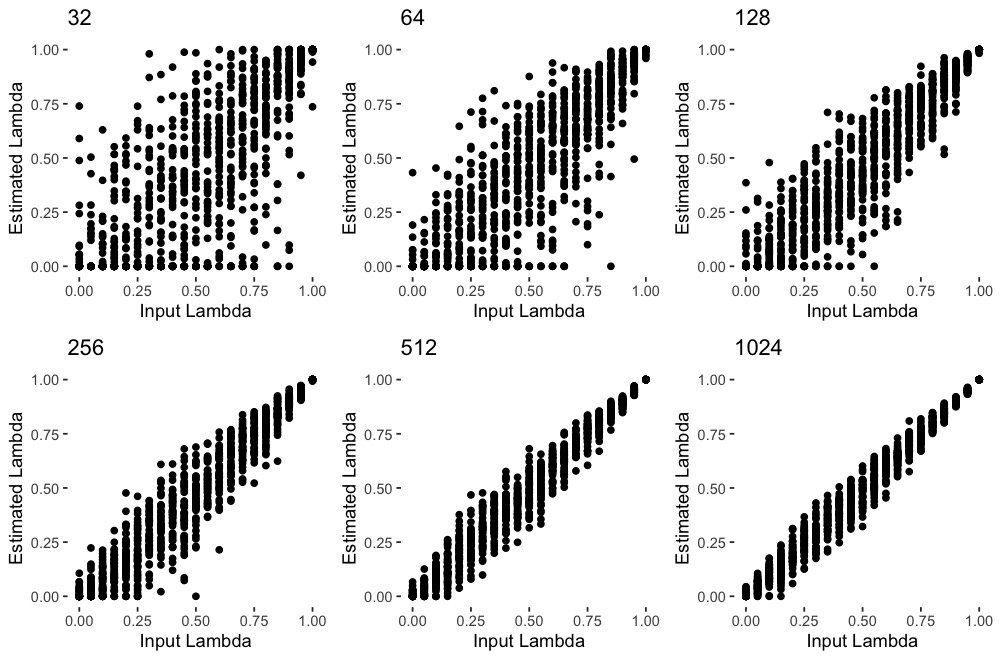
\includegraphics[width=0.95\linewidth]{Fig1}

\singlespacing \textbf{Figure 1}. Accuracy of Pagel's lambda estimations
across known lambda inputs on various tree sizes. As trees increase in
size, the estimates more closely resemble the input lambdas, however
considerable and concerning variation is apparent in trees smaller than
those with 256 tips. \hfill\break

\newpage

\section{Other Figures Here}\label{other-figures-here}

\end{document}
